\section{Die Toolbox}\raggedbottom %TODO besserer Titel
\subsection{Typen}
Die Toolbox 1.0 konnte mit Grammatiken und Automaten umgehen. Hierzu geh�ren
insbesondere, aber nicht ausschlie�lich
\begin{itemize}
  \item die Entwicklung eines eigenen Datentypes f�r Grammatiken und Automaten
  \item das Parsen von Grammatiken und Automaten mittels SableCC\footnote{hier
  Referenz}
  \item das Speichern von Grammatiken und Automaten in Datein
  \item First- und Follow-Set einer Grammatik
  \item Vervollst�ndigung und Entfernen von$\lambda$-�berg�ngen von Automaten
\end{itemize}
\subsection{Erweiterbarkeit}
Das von Herrn Ruhland entwickelte System legt Wert darauf, leicht
weiterentwickelbar zu sein. Hierf�r wurde ein Plugin-System entwickelt, das es
einem anderen Programmieren erleichtert, neue Features hinzu zu entwickeln,
ohne sich mit dem bereits bestehenden Code vertraut zu machen.
Es gibt hierbei verschiedene Arten von Plugins, die automatisch eingebunden
werden
\begin{itemize}
  \item CLI-Plugins - Kommandozeilenprogramme
  \item SimpleFunction Plugins - GUI-Funktionen, die keine Nutzereingabe
  ben�tigen.
  \item ComplexFunction Plugins - GUI-Funktionen, die Nutzerinteraktion
  ben�tigen
  \item DisplayPlugins - werden dazu benutzt, Datentypen darzustellen
\end{itemize}
\subsection{Mechanismen}
Das Programm sollte sowohl �ber die Konsole als auch �ber eine Benutzeroberfl�che bedient werden k�nnen.
Hierf�r gibt es die beiden zentralen Klassen \textit{CLI} f�r die Konsole und \textit{GUI} f�r die grafische Benutzeroberfl�che.
Die Plugins haben die Methoden \textit{getInputType} und \textit{getOutputType}. Diese lieferen eine Klasse,
von der das Plugin eine Instanz als Eingabe bekommt bzw. als Ausgabe zur�ckgibt.
Sobald der Nutzer ein Kommando in der Konsole (oder der GUI) durchf�hrt, ruft
die Klasse CLI (oder die Klasse GUI) die \textit{execute}-Methode des jeweiligen
Plugins auf und �bergibt das aktuelle Objektder passende Klassen.
Von jeder Klasse ist immer nur ein Objekt gespeichert.
Das von der \textit{execute}-Methode zur�ckgelieferte Objekt �berschreibt das
bisherige.
\subsection{GUI}
Dies ist die Benutzeroberfl�che der Toolbox 1.0 im Grammar-Modus. Die aktuelle Grammatik wird zum Bearbeiten angezeigt. Um Automaten zu bearbeiten, muss man unter \textit{Choose Plugin} \textit{Automaton} w�hlen.
\begin{figure}[hbtp]
	\centering
	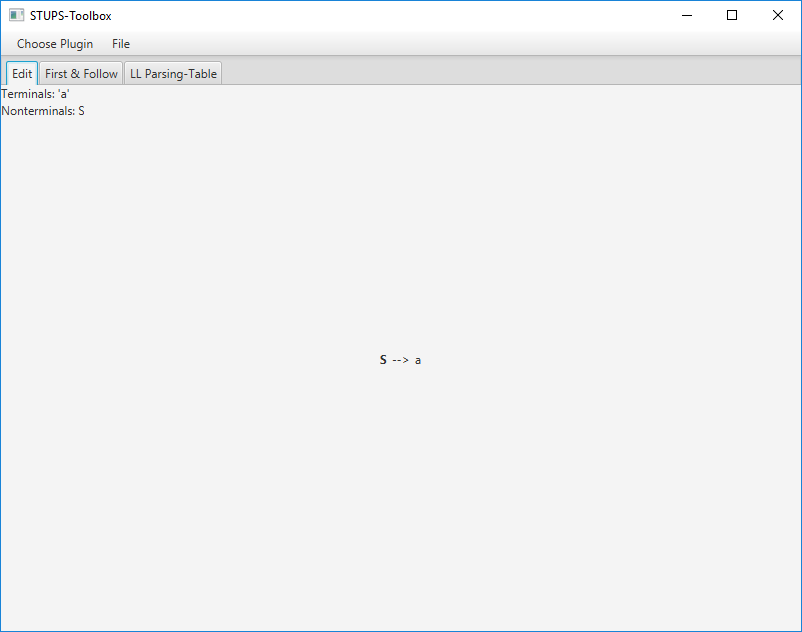
\includegraphics[width=1\textwidth]{bilder/gui_alt.png}
	\caption{Die GUI der Toolbox 1.0}
	\label{img:oldgui}
\end{figure}

